\chapter{Processo Escolhido}
\label{chosen-process}

\section{Imagens do Processo a ser Utilizado}

\begin{figure}[htb]
\centering
  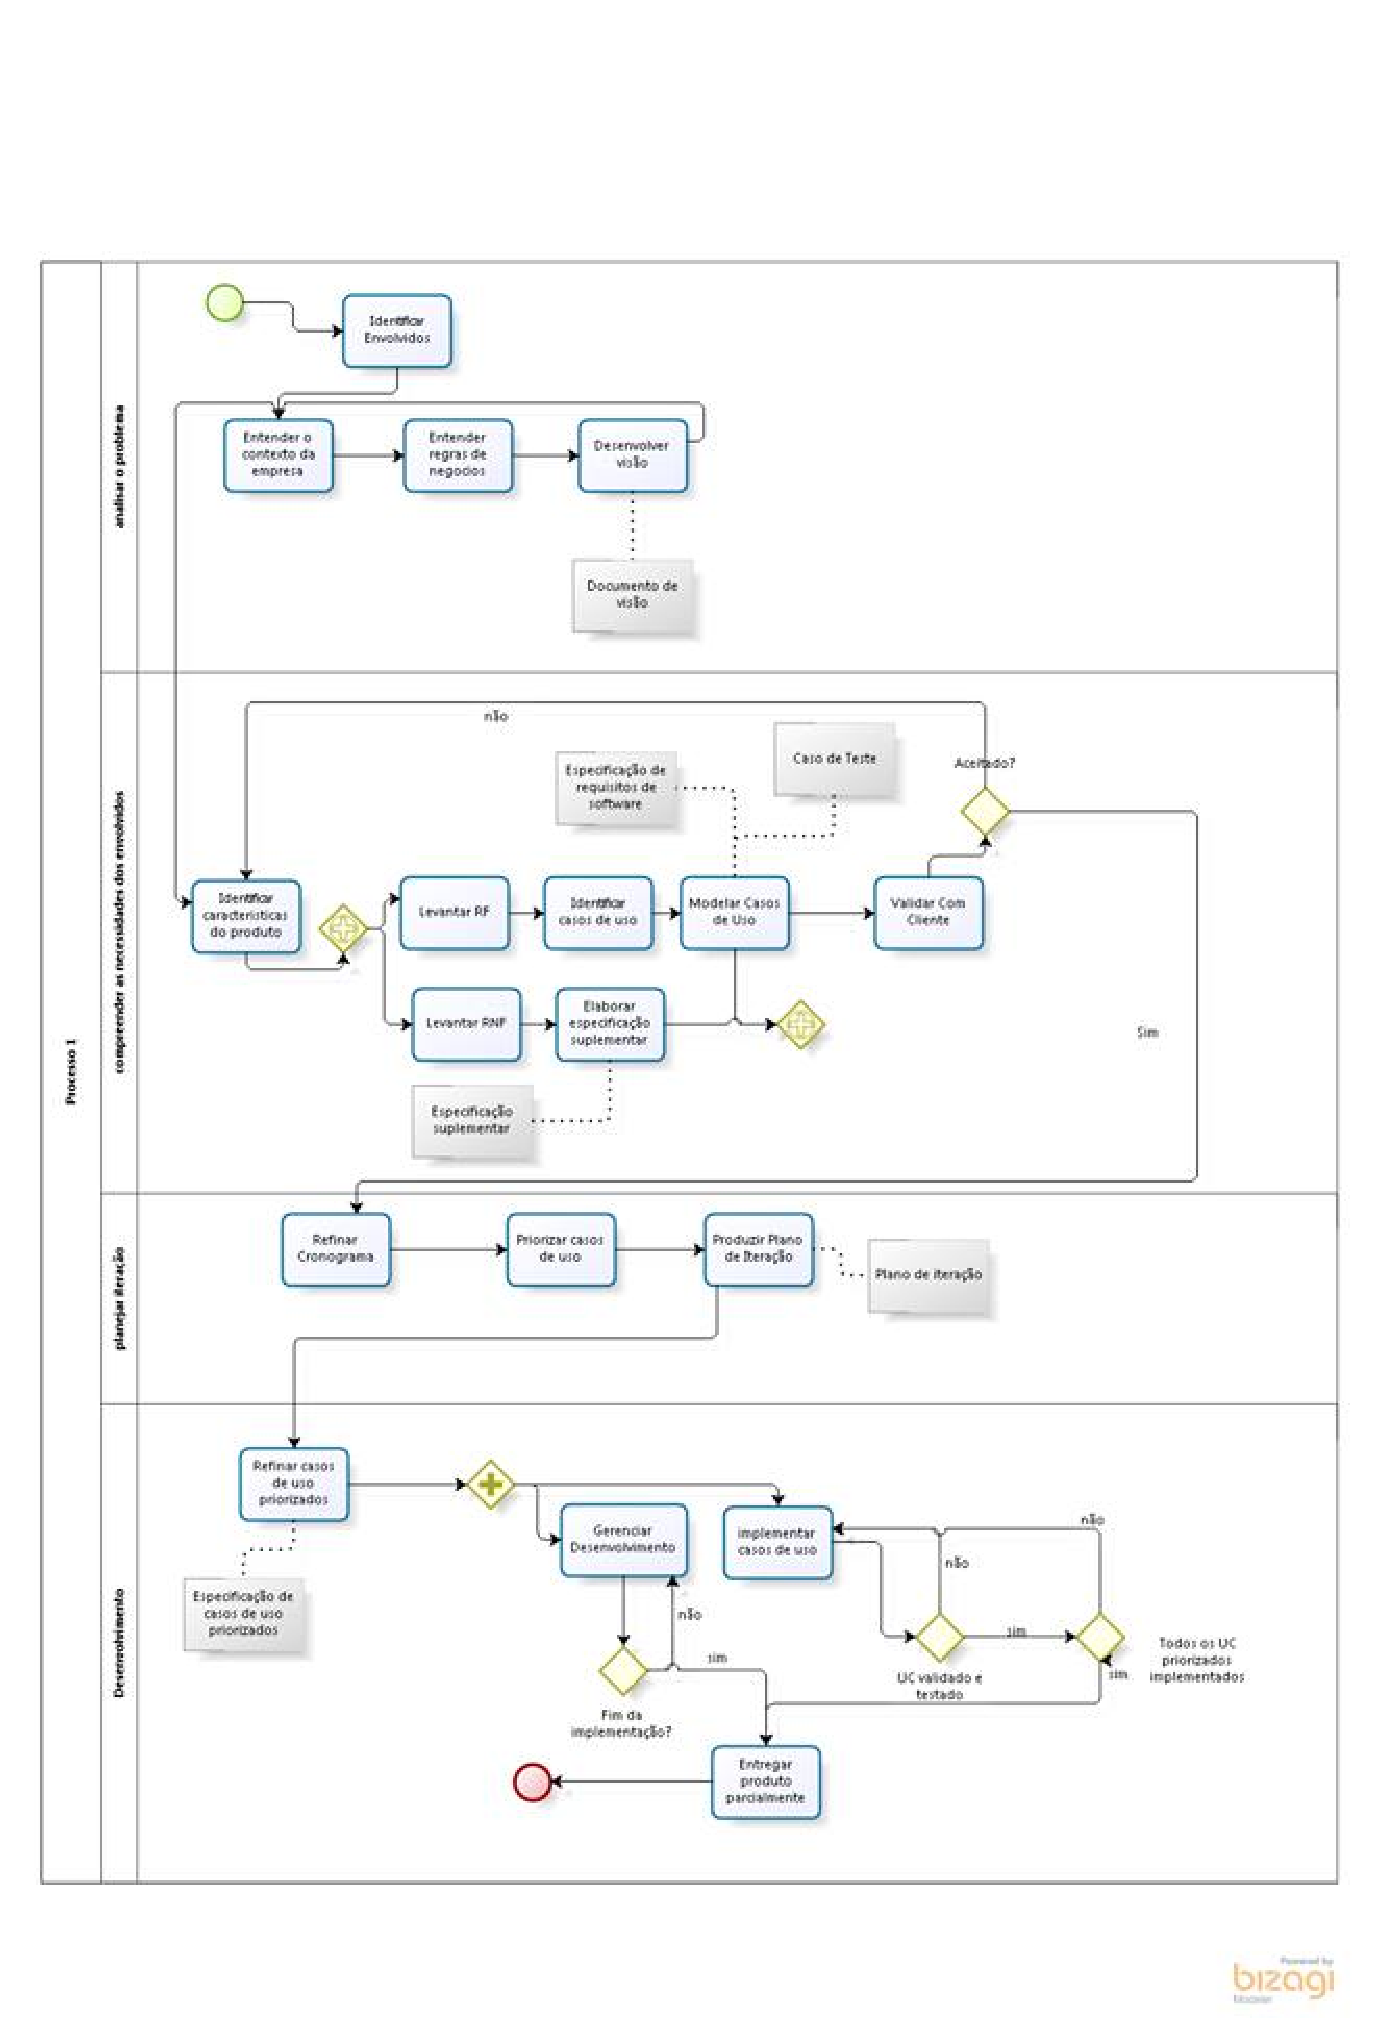
\includegraphics[keepaspectratio=true,scale=0.5]
  {figuras/processo_todo.eps}
  \caption{Processo Adotado}
  \label{process}
\end{figure}

\begin{figure}[htb]
\centering
 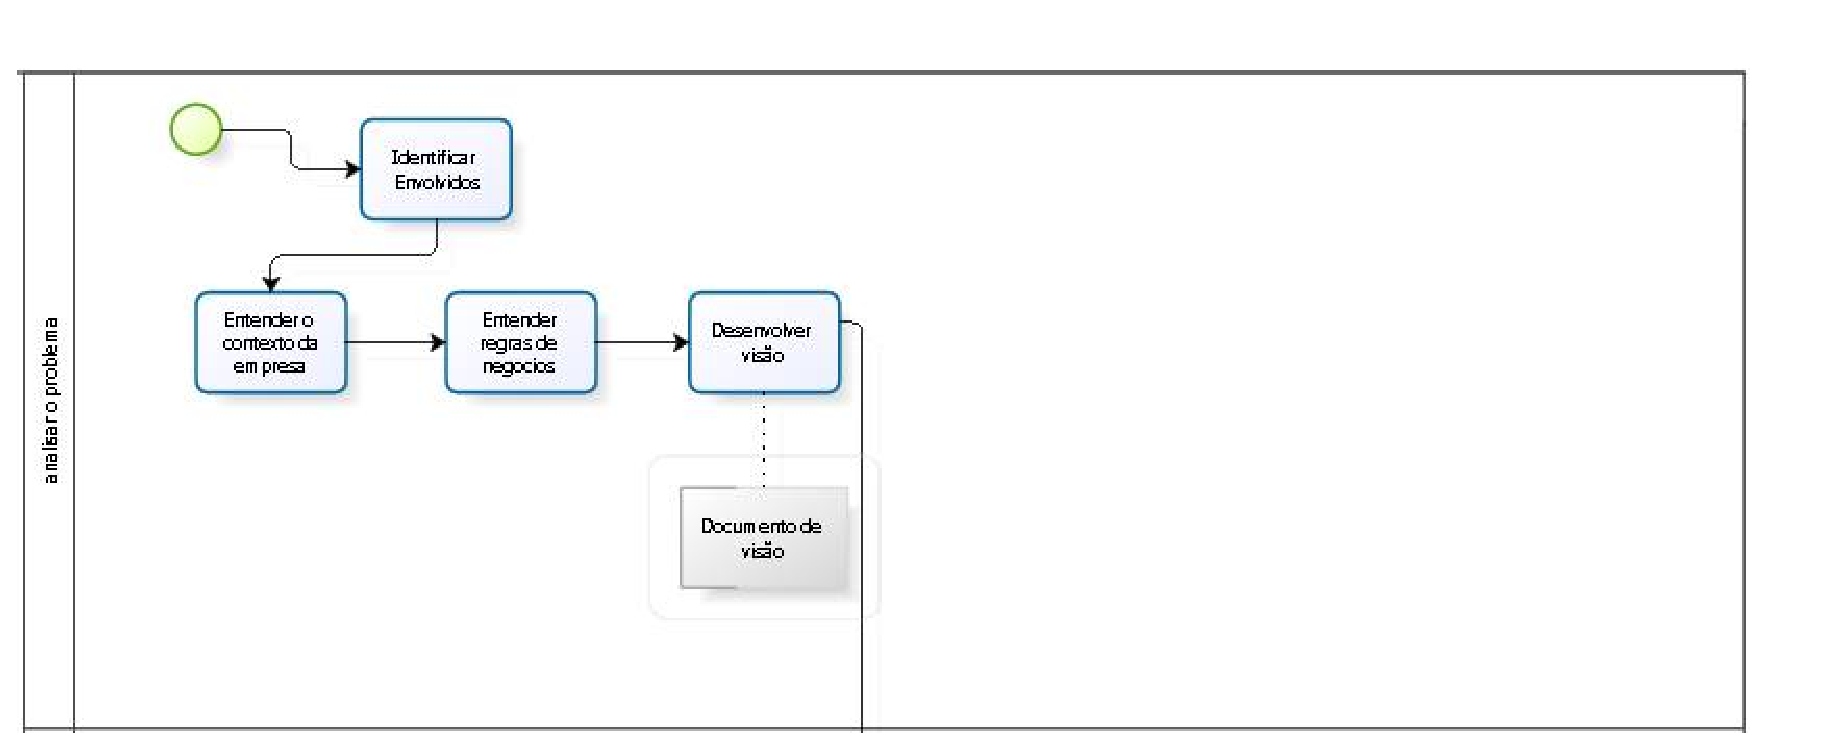
\includegraphics[keepaspectratio=true,scale=0.6]
  {figuras/analisar_problema.eps}
  \caption{\textit{Line} analisar o problema}
  \label{analyze}
\end{figure}

\begin{figure}[htb]
\centering
  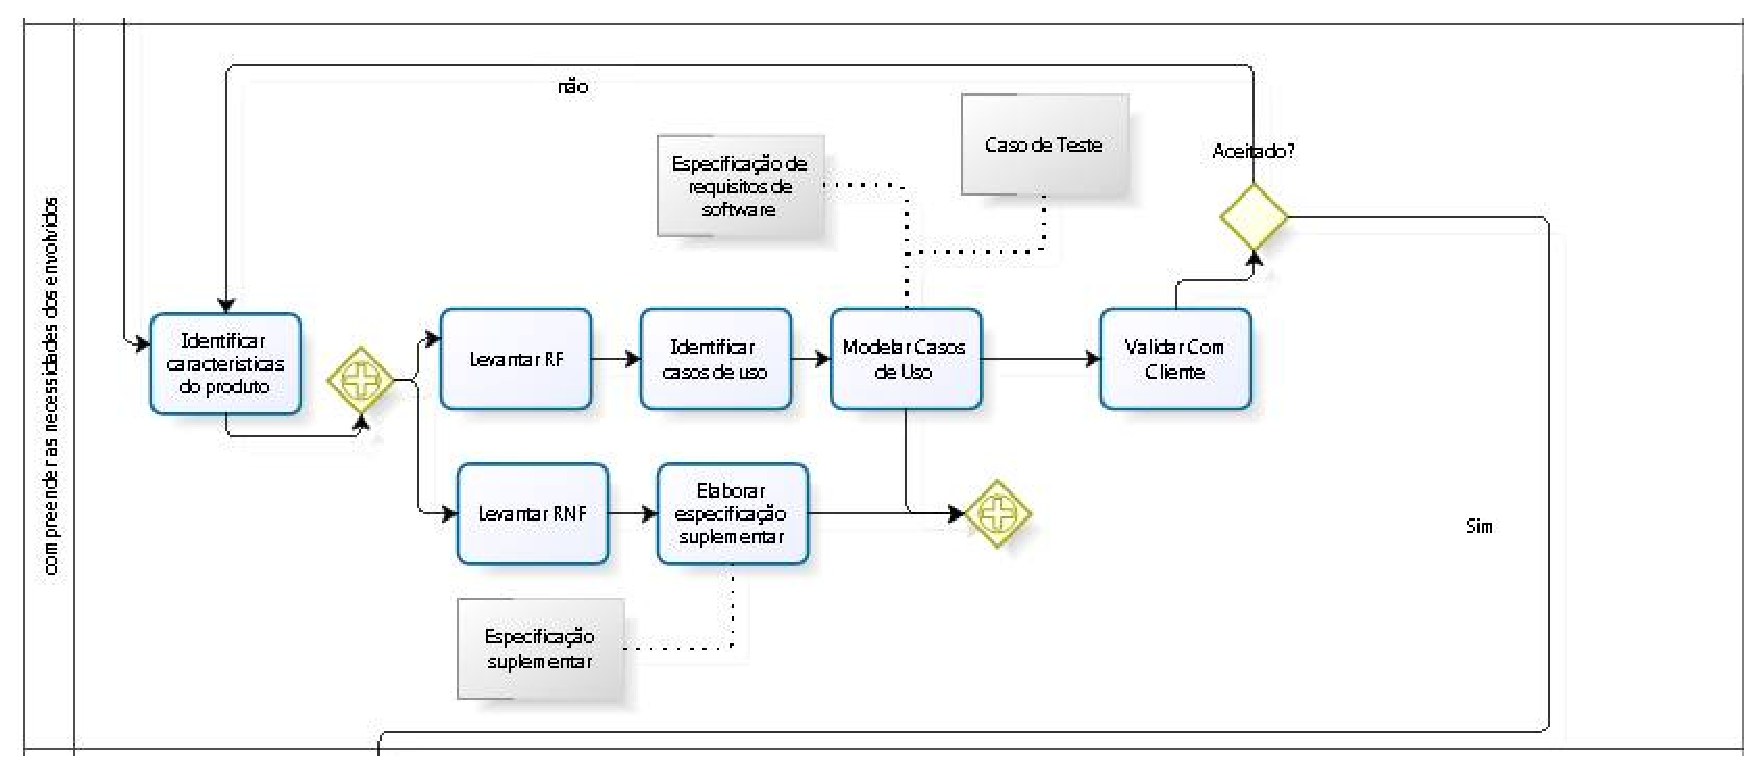
\includegraphics[keepaspectratio=true,scale=0.6]
  {figuras/compreender.eps}
  \caption{\textit{Line} compreender as necessidades dos envolvidos}
  \label{comprehend}
\end{figure}

\begin{figure}[htb]
\centering
  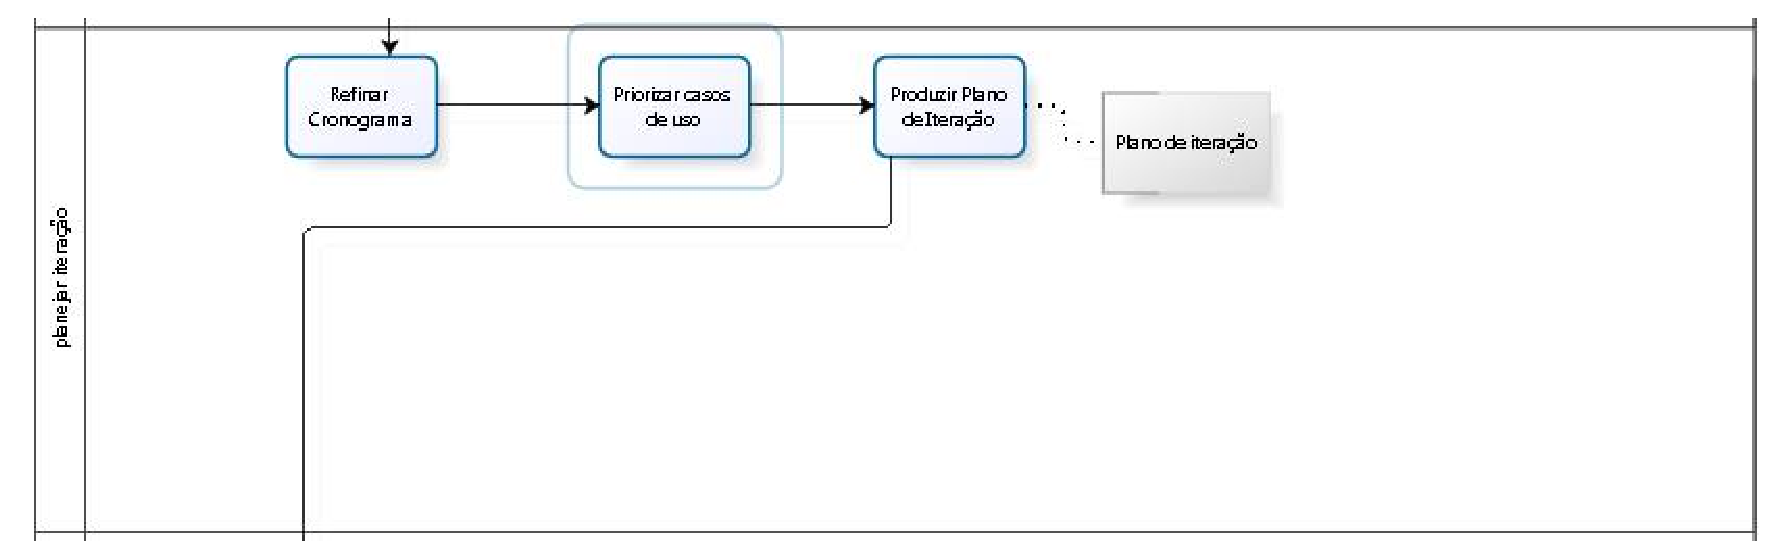
\includegraphics[keepaspectratio=true,scale=0.6]
  {figuras/planejar.eps}
  \caption{\textit{Line} planejar iteração}
  \label{planning}
\end{figure}

\begin{figure}[htb]
\centering
  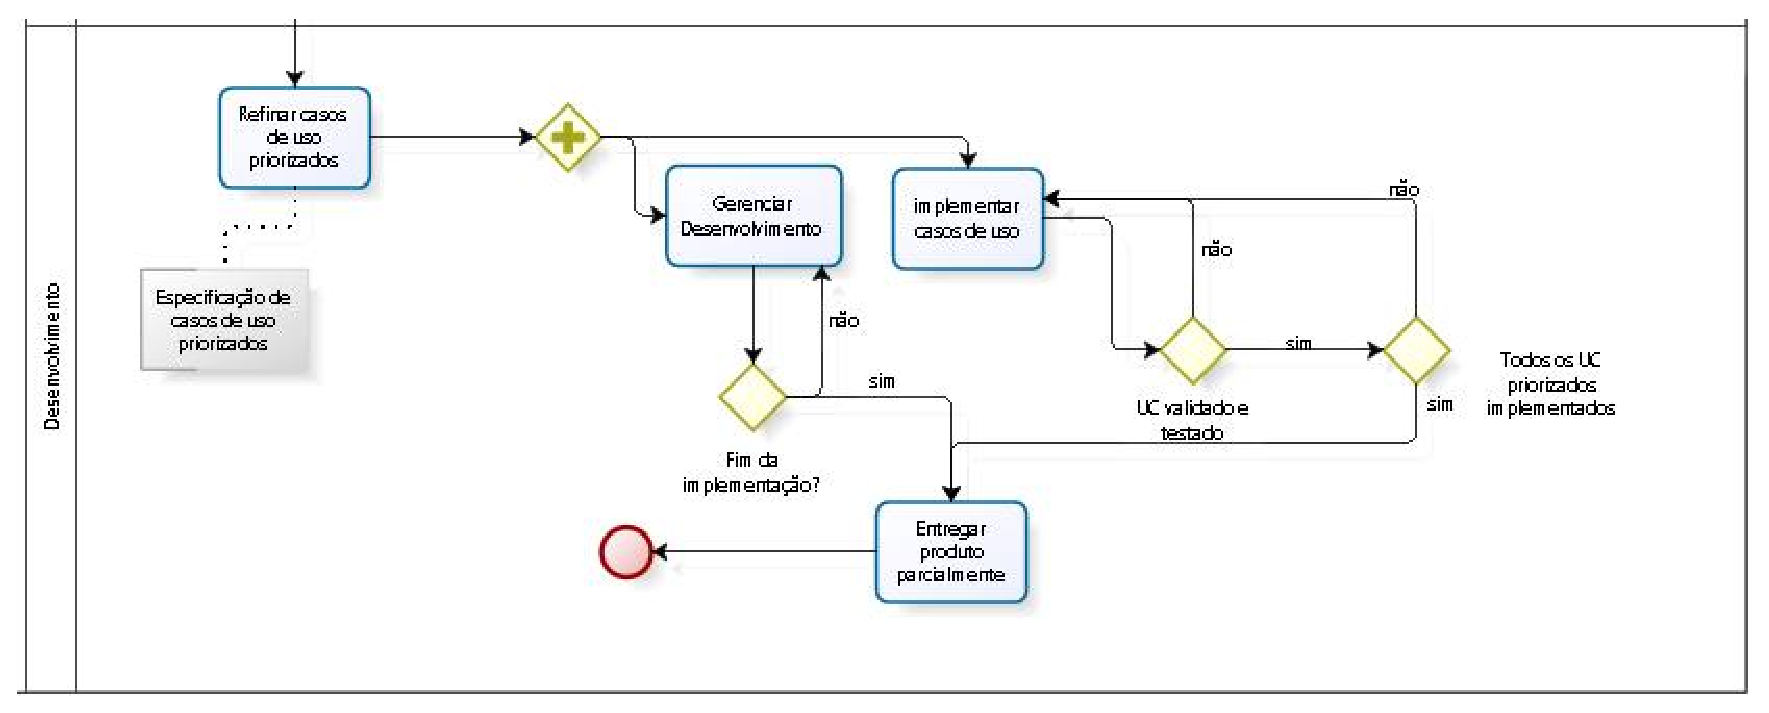
\includegraphics[keepaspectratio=true,scale=0.6]
  {figuras/desenvolvimento.eps}
  \caption{\textit{Line} desenvolvimento}
  \label{devel}
\end{figure}

\clearpage{}

\section{Descrição das Atividades do Processo}

\subsection{Analisar o Problema}

\subsubsection{Identificar Envolvidos}

\begin{itemize}
\item \textbf{Descrição}: Identificar quem são todas as pessoas envolvidas no processo de desenvolvimento
\item \textbf{Tarefas}: Entrevistas
\item \textbf{Resultados esperados do MPS-BR}: Nenhum
\item \textbf{Atividade da Engenharia de Requisitos}: Elicitação de Requisitos e Documentação
\item \textbf{Artefatos de entrada}: Nenhum
\item \textbf{Artefatos gerados ou alterados}: Documento especificando todos os \textit{stakeholders} e atores do sistema
\end{itemize}

\subsubsection{Entender o Contexto da Empresa}

\begin{itemize}
\item \textbf{Descrição}: Compreender como é o funcionamento da empresa e seu atual processo
\item \textbf{Tarefas}: Entrevistas, Observações e Cenários
\item \textbf{Resultados esperados do MPS-BR}: Nenhum
\item \textbf{Atividade da Engenharia de Requisitos}: Elicitação de requisitos e Documentação
\item \textbf{Artefatos de entrada}: Nenhum
\item \textbf{Artefatos gerados ou alterados}: Documento explicando resumidamente o processo da empresa
\end{itemize}

\subsubsection{Entender Regras de Negócios}

\begin{itemize}
\item \textbf{Descrição}: Especificar quais são as regras que regem o modo como a empresa opera
\item \textbf{Tarefas}: Entrevistas e cenários
\item \textbf{Resultados esperados do MPS-BR}: Nenhum
\item \textbf{Atividade da Engenharia de Requisitos}: Elicitação de Requisitos e Documentação
\item \textbf{Artefatos de entrada}: Nenhum
\item \textbf{Artefatos gerados ou alterados}: Documento de especificação de regras de negócios
\end{itemize}

\subsubsection{Desenvolver Documento de Visão}

\begin{itemize}
\item \textbf{Descrição}: Condensar as informações levantadas nos passos anteriores e novas informações em uma visão geral sobre o produto a ser desenvolvido
\item \textbf{Tarefas}: Entrevistas, observação e cenários
\item \textbf{Resultados esperados do MPS-BR}: Nenhum
\item \textbf{Atividade da Engenharia de Requisitos}: Elicitação de Requisitos e Documentação
\item \textbf{Artefatos de entrada}: Documento de contexto, regras de negócio e de \textit{stakeholders}
\item \textbf{Artefatos gerados ou alterados}: Documento de Visão
\end{itemize}

\begin{description}
\item\textbf{Descrição}: Identificar quem são todas as pessoas envolvidas no processo de desenvolvimento
\item\textbf{Tarefas}: Entrevistas
\item\textbf{Resultados esperados do MPS-BR}: Nenhum
\item\textbf{Atividade da Engenharia de Requisitos}: Elicitação de Requisitos e Documentação
\item\textbf{Artefatos de entrada}: Nenhum
\item\textbf{Artefatos gerados ou alterados}: Documento especificando todos os \textit{stakeholders}
\end{description}

\subsubsection{Entender o Contexto da Empresa}

\begin{description}
\item\textbf{Descrição}: Compreender como é o funcionamento da empresa e seu atual processo
\item\textbf{Tarefas}: Entrevistas, Observações e Cenários
\item\textbf{Resultados esperados do MPS-BR}: Nenhum
\item\textbf{Atividade da Engenharia de Requisitos}: Elicitação de Requisitos e Documentação
\item\textbf{Artefatos de entrada}: Nenhum
\item\textbf{Artefatos gerados ou alterados}: Documento explicando resumidamente a forma de atuação da empresa
\end{description}

\subsubsection{Entender Regras de Negócios}

\begin{description}
\item\textbf{Descrição}: Especificar quais são as regras que regem o modo como a empresa opera
\item\textbf{Tarefas}: Entrevistas e Cenários
\item\textbf{Resultados esperados do MPS-BR}: Nenhum
\item\textbf{Atividade da Engenharia de Requisitos}: Elicitação de Requisitos e Documentação
\item\textbf{Artefatos de entrada}: Nenhum
\item\textbf{Artefatos gerados ou alterados}: Documento de Especificação de Regras de Negócios
\end{description}

\subsubsection{Desenvolver Documento de Visão}

\begin{description}
\item\textbf{Descrição}: Condensar as informações levantadas nas atividades anteriores e novas informações em uma visão geral sobre o produto a ser desenvolvido
\item\textbf{Tarefas}: Entrevistas, Observação e Cenários
\item\textbf{Resultados esperados do MPS-BR}: Nenhum
\item\textbf{Atividade da Engenharia de Requisitos}: Elicitação de Requisitos e Documentação
\item\textbf{Artefatos de entrada}: Documento de contexto, regras de negócio e de \textit{stakeholders}
\item\textbf{Artefatos gerados ou alterados}: Documento de Visão
\end{description}

\subsection{Compreender Necessidade dos Envolvidos}

\subsubsection{Identificar Características do Produto}

\begin{itemize}
\item \textbf{Descrição}: Identificar as características do produto com alto nível de abstração
\item \textbf{Tarefas}: Entrevistas, observações e cenários
\item \textbf{Resultados esperados do MPS-BR}: GRE-1 e DRE-1
\item \textbf{Atividade da Engenharia de Requisitos}: Análise e Negociação
\item \textbf{Artefatos de entrada}: Temas de Investimento e Solicitação dos Envolvidos
\item \textbf{Artefatos gerados ou alterados}: Relato sobre o Produto, Requisitos Funcionais e Requisitos Não Funcionais
\end{itemize}

\subsubsection{Levantar RF e RNF}

\begin{itemize}
\item \textbf{Descrição}: Identificar as características funcionais e não funcionais do produto
\item \textbf{Tarefas}: Entrevistas e refinar atributos dos requisitos
\item \textbf{Resultados esperados do MPS-BR}: GRE-1, DRE-1, DRE-7
\item \textbf{Atividade da Engenharia de Requisitos}:  Elicitação, Análise e Negociação, Documentação e Gerência de Requisitos
\item \textbf{Artefatos de entrada}: Temas de Investimento e Solicitação dos Envolvidos
\item \textbf{Artefatos gerados ou alterados}: Requisitos Funcionais, Requisitos Não Funcionais e Plano de Gerência de Requisitos
\end{itemize}

\subsubsection{Identificar Casos de Uso}

\begin{itemize}
\item \textbf{Descrição}: Capturar os requisitos do sistema que agregarão valor ao cliente
\item \textbf{Tarefas}: Identificar atores e Identificar Requisitos Funcionais
\item \textbf{Resultados esperados do MPS-BR}: GRE-3 e DRE-4
\item \textbf{Atividade da Engenharia de Requisitos}: Verificação e Validação
\item \textbf{Artefatos de entrada}: Requisitos Funcionais
\item \textbf{Artefatos gerados ou alterados}: Modelo de Casos de Uso e Diagrama de Casos de Uso
\end{itemize}

\subsubsection{Elaborar Especificação Suplementar}

\begin{itemize}
\item \textbf{Descrição}: Capturar os requisitos do sistema que não são identificados imediatamente no modelo de casos de uso
\item \textbf{Tarefas}: Identificar Requisitos Não Funcionais
\item \textbf{Resultados esperados do MPS-BR}: GRE-3, DRE-3, DRE-4 e DRE-7
\item \textbf{Atividade da Engenharia de Requisitos}: Verificação e Validação
\item \textbf{Artefatos de entrada}: Requisitos Não Funcionais
\item \textbf{Artefatos gerados ou alterados}: Especificação Suplementar
\end{itemize}

\subsubsection{Modelar Casos de Uso}

\begin{itemize}
\item \textbf{Descrição}: Com base nos requisitos do \textit{software}, são criados os Casos de Uso e respectivos Diagramas de Caso de Uso e seus Casos de Teste
\item \textbf{Tarefas}: Descrever os Casos de Uso bem como seus diagramas e Casos de Teste
\item \textbf{Resultados esperados do MPS-BR}: GRE-2, DRE-2, DRE-3, DRE-5 e DRE-6
\item \textbf{Atividade da Engenharia de Requisitos}: Documentação
\item \textbf{Artefatos de entrada}: Requisitos Funcionais
\item \textbf{Artefatos gerados ou alterados}: Especificação de Requisitos de \textit{Software} e Casos de Teste
\end{itemize}

\subsubsection{Validar com o Cliente}

\begin{itemize}
\item \textbf{Descrição}: Valida com o cliente se os requisitos elicitados e os casos de uso documentados condizem com as suas expectativas
\item \textbf{Tarefas}: Validar com o cliente os Requisitos Funcionais, Não Funcionais e Casos de Uso
\item \textbf{Resultados esperados do MPS-BR}: GRE-2, GRE-4, GRE-5 e DRE-8
\item \textbf{Atividade da Engenharia de Requisitos}: Verificação e Validação
\item \textbf{Artefatos de entrada}: Requisitos Funcionais, Não Funcionais e Casos de Uso
\item \textbf{Artefatos gerados ou alterados}: Reinicia o ciclo de desenvolvimento caso seja reprovado pelo cliente. Em cenário de aprovação, nada é alterado
\end{itemize}

\begin{description}
\item\textbf{Descrição}: Identificar as características do produto com alto nível de abstração
\item\textbf{Tarefas}: Entrevistas, Observações e Cenários
\item\textbf{Resultados esperados do MPS-BR}: GRE-1 e DRE-1
\item\textbf{Atividade da Engenharia de Requisitos}: Análise e Negociação
\item\textbf{Artefatos de entrada}: Temas de Investimento e Solicitação dos Envolvidos
\item\textbf{Artefatos gerados ou alterados}: Relato sobre o Produto, Requisitos Funcionais e Requisitos Não Funcionais
\end{description}

\subsubsection{Levantar RF e RNF}

\begin{description}
\item\textbf{Descrição}: Identificar os requisitos funcionais e não funcionais do produto
\item\textbf{Tarefas}: Entrevistas e refinar atributos dos requisitos
\item\textbf{Resultados esperados do MPS-BR}: GRE-1, DRE-1, DRE-7
\item\textbf{Atividade da Engenharia de Requisitos}:  Elicitação, Análise e Negociação, Documentação e Gerência de Requisitos
\item\textbf{Artefatos de entrada}: Temas de Investimento e Solicitação dos Envolvidos
\item\textbf{Artefatos gerados ou alterados}: Requisitos Funcionais, Requisitos Não Funcionais e Plano de Gerência de Requisitos
\end{description}

\subsubsection{Identificar Casos de Uso}

\begin{description}
\item\textbf{Descrição}: Capturar os requisitos do sistema que agregarão valor ao cliente
\item\textbf{Tarefas}: Identificar atores e Identificar Requisitos Funcionais
\item\textbf{Resultados esperados do MPS-BR}: GRE-3 e DRE-4
\item\textbf{Atividade da Engenharia de Requisitos}: Verificação e Validação
\item\textbf{Artefatos de entrada}: Requisitos Funcionais
\item\textbf{Artefatos gerados ou alterados}: Modelo de Casos de Uso e Diagrama de Casos de Uso
\end{description}

\subsubsection{Elaborar Especificação Suplementar}

\begin{description}
\item\textbf{Descrição}: Capturar os requisitos do sistema que não são identificados imediatamente no modelo de casos de uso
\item\textbf{Tarefas}: Identificar Requisitos Não Funcionais
\item\textbf{Resultados esperados do MPS-BR}: GRE-3, DRE-3, DRE-4 e DRE-7
\item\textbf{Atividade da Engenharia de Requisitos}: Verificação e Validação
\item\textbf{Artefatos de entrada}: Requisitos Não Funcionais
\item\textbf{Artefatos gerados ou alterados}: Especificação Suplementar
\end{description}

\subsubsection{Modelar Casos de Uso}

\begin{description}
\item\textbf{Descrição}: Com base nos requisitos do \textit{software}, são criados os Casos de Uso e respectivos Diagramas de Caso de Uso e seus Casos de Teste
\item\textbf{Tarefas}: Descrever os Casos de Uso bem como seus diagramas e Casos de Teste
\item\textbf{Resultados esperados do MPS-BR}: GRE-2, DRE-2, DRE-3, DRE-5 e DRE-6
\item\textbf{Atividade da Engenharia de Requisitos}: Documentação
\item\textbf{Artefatos de entrada}: Requisitos Funcionais
\item\textbf{Artefatos gerados ou alterados}: Especificação de Requisitos de \textit{Software} e Casos de Teste
\end{description}

\subsubsection{Validar com o Cliente}

\begin{description}
\item\textbf{Descrição}: Valida com o cliente se os requisitos elicitados e os casos de uso documentados condizem com as suas expectativas
\item\textbf{Tarefas}: Validar com o cliente os Requisitos Funcionais, Não Funcionais e Casos de Uso
\item\textbf{Resultados esperados do MPS-BR}: GRE-2, GRE-4, GRE-5 e DRE-8
\item\textbf{Atividade da Engenharia de Requisitos}: Verificação e Validação
\item\textbf{Artefatos de entrada}: Requisitos Funcionais, Não Funcionais e Casos de Uso
\item\textbf{Artefatos gerados ou alterados}: Reinicia o ciclo de desenvolvimento caso seja reprovado pelo cliente. Em cenário de aprovação, nada é alterado
\end{description}

\subsection{Planejar Iteração}

\subsubsection{Refinar Cronograma}

\begin{description}
\item\textbf{Descrição}: Rever e atualizar o cronograma do projeto
\item\textbf{Tarefas}: Manter o cronograma consistente com o andamento do projeto
\item\textbf{Resultados esperados do MPS-BR}: GRE-4
\item\textbf{Atividade da Engenharia de Requisitos}: Gerência de Requisitos
\item\textbf{Artefatos de entrada}: Cronograma de Projeto
\item\textbf{Artefatos gerados ou alterados}: Cronograma de Projeto atualizado
\end{description}

\subsubsection{Priorizar Casos de Uso}

\begin{description}
\item\textbf{Descrição}: Escolher quais casos de uso serão implementados
\item\textbf{Tarefas}: Escolher os casos de uso a serem implementados de acordo com as prioridades e pré-requisitos
\item\textbf{Resultados esperados do MPS-BR}: DRE-2
\item\textbf{Atividade da Engenharia de Requisitos}: Gerência de Requisitos
\item\textbf{Artefatos de entrada}: Casos de Uso e Casos de Teste
\item\textbf{Artefatos gerados ou alterados}: Casos de Uso priorizados serão descritos no Plano de Iteração
\end{description}

\subsubsection{Produzir Plano de Iteração}

\begin{description}
\item\textbf{Descrição}: Descrever quais casos de uso foram priorizados para a iteração
\item\textbf{Tarefas}: Produzir o artefato de Plano de Iteração
\item\textbf{Resultados esperados do MPS-BR}: DRE-2
\item\textbf{Atividade da Engenharia de Requisitos}: Gerência de Requisitos
\item\textbf{Artefatos de entrada}: Casos de Uso e Casos de Teste
\item\textbf{Artefatos gerados ou alterados}: Plano de Iteração
\end{description}

\subsection{Implementação}

\subsubsection{Refinar Casos de Uso Priorizados}


\begin{description}
\item\textbf{Descrição}: Validar os casos de uso com o cliente para garantir que todos os atributos dos casos de uso estão de acordo com a necessidade do cliente
\item\textbf{Tarefas}: Validar Casos de Uso com o cliente e detalhar Casos de Uso
\item\textbf{Resultados esperados do MPS-BR}: GRE-4, DRE-3, DRE-4, DRE-7, DRE-8
\item\textbf{Atividade da Engenharia de Requisitos}: Análise e Negociação
\item\textbf{Artefatos de entrada}: Diagrama de Casos de Uso e Modelo de Casos de Uso
\item\textbf{Artefatos gerados ou alterados}: Diagrama de Casos de Uso, Modelo de Casos de Uso, Especificação de Requisitos de \textit{Software}
\end{description}

\subsubsection{Implementar Casos de Uso}

\begin{description}
\item\textbf{Descrição}: Implementar os Casos de Uso que foram descritos na Especificação de Requisitos de \textit{Software}
\item\textbf{Tarefas}: Implementar parte da solução, com base na Especificação de Requisitos de \textit{Software} e validar implementação de Caso de Uso com o cliente
\item\textbf{Resultados esperados do MPS-BR}: Nenhum
\item\textbf{Atividade da Engenharia de Requisitos}: Nenhuma
\item\textbf{Artefatos de entrada}: Diagrama de Casos de Uso, Modelo de Caso de Uso e Especificação de Caso de Uso
\item\textbf{Artefatos gerados ou alterados}: Nenhum
\end{description}

\subsubsection{Gerenciar Desenvolvimento}

\begin{description}
\item\textbf{Descrição}: Verificar se as atividades da ER estão de acordo com a visão do cliente
\item\textbf{Tarefas}: Revisar os requisitos e gerenciar dependências
\item\textbf{Resultados esperados do MPS-BR}: GRE-3, GRE-4, GRE-5
\item\textbf{Atividade da Engenharia de Requisitos}: Gerenciar Requisitos
\item\textbf{Artefatos de entrada}: Diagrama de Casos de Uso, Modelo de Casos de Uso e Documento de Visão
\item\textbf{Artefatos gerados ou alterados}: Nenhum
\end{description}

\subsubsection{Entregar Produto}

\begin{description}
\item\textbf{Descrição}: Entregar parte da solução para o cliente, indicando o fim do ciclo de vida do projeto
\item\textbf{Tarefas}: Revisar os requisitos e gerenciar dependências
\item\textbf{Resultados esperados do MPS-BR}: Nenhum
\item\textbf{Atividade da Engenharia de Requisitos}: Nenhuma
\item\textbf{Artefatos de entrada}: Diagrama de Casos de Uso, Modelo de Casos de Uso e Documento de Visão
\item\textbf{Artefatos gerados ou alterados}: Nenhum
\end{description}

\section{Papéis}

\subsection{Gerente de Controle de Mudanças}

\textbf{Definição}
\begin{itemize}
\item Supervisiona o controle de mudanças, geralmente formado por um conjunto entre todos os envolvidos
\end{itemize}

\textbf{Responsável por}
\begin{itemize}
\item Estabelecer processo de controle de mudanças
\item Revisar solicitação de mudanças
\item Confirmar se há duplicidade entre as solicitações
\end{itemize}

\textbf{Artefato gerado ou alterado}
\begin{itemize}
\item Solicitação de Mudança
\end{itemize}

\subsection{Gerente de Projeto}

\textbf{Definição}
\begin{itemize}
\item Aloca recursos, ajusta prioridades, coordena interações com clientes e mantém a equipe focada em uma meta específica
\end{itemize}

\textbf{Responsável por}
\begin{itemize}
\item Caso de Negócio
\item Métricas do Projeto
\item Iniciar o Projeto
\end{itemize}

\textbf{Artefato gerado ou alterado}
\begin{itemize}
\item Caso de Negócio
\end{itemize}

\subsection{Analista de Processos de Negócios}

\textbf{Definição}
\begin{itemize}
\item Lidera e coordena a modelagem de casos de uso de negócios, definindo e delimitando a organização que está sendo modelada
\end{itemize}

\textbf{Responsável por}
\begin{itemize}
\item Estabelece quais são os atores e casos de uso de negócio
\item Capturar vocabulário comum
\item Estruturar Modelo de Casos de Uso de Negócios
\end{itemize}

\textbf{Artefato gerado ou alterado}
\begin{itemize}
\item Glossário
\item Especificação Suplementar de negócios
\item Modelo de Caso de Uso de Negócios
\end{itemize}

\subsection{Analista de Sistemas}

\textbf{Definição}
\begin{itemize}
\item Lidera e coordena a identificação de requisitos e a Modelagem de Casos de Uso, delimitando o sistema e definindo suas funcionalidades
\end{itemize}

\textbf{Responsável por}
\begin{itemize}
\item Desenvolver Plano de Gerência de Requisitos
\item Desenvolver Visão
\item Identificar Solicitação dos Envolvidos
\item Identificar Atores e Casos de Uso
\end{itemize}

\textbf{Artefato gerado ou alterado}
\begin{itemize}
\item Plano de Gerência de Requisitos
\item Visão
\item Atributos de Requisitos
\item Solicitação dos Envolvidos
\end{itemize}

\subsection{\textit{Designer} de Negócios}

\textbf{Definição}
\begin{itemize}
\item Detalha a especificação de uma parte da organização, descrevendo o fluxo de trabalho de um ou de vários casos de uso de negócios
\end{itemize}

\textbf{Responsável por}
\begin{itemize}
\item Detalhar Casos de Uso de Negócios
\end{itemize}

\textbf{Artefato gerado ou alterado}
\begin{itemize}
\item Casos de Uso de Negócios
\end{itemize}

\subsection{Especificador de Requisitos}

\textbf{Definição}
\begin{itemize}
\item Detalha a especificação de uma parte da funcionalidade do sistema, descrevendo os requisitos de um ou vários casos de uso
\end{itemize}

\textbf{Responsável por}
\begin{itemize}
\item Detalhar Casos de Uso
\item Detalhar Requisitos de \textit{Software}
\end{itemize}

\textbf{Artefato gerado ou alterado}
\begin{itemize}
\item Casos de Uso
\item Especificação de Requisitos
\end{itemize}
